\documentclass[12pt,a4paper]{article}

% ---- Packages ----
\usepackage{amsmath,amssymb,amsthm,mathtools}
\usepackage{tikz-cd}
\usepackage{tikz}
\usetikzlibrary{arrows.meta,positioning,shapes.geometric,fit,backgrounds,calc}
\usepackage[colorlinks=true,linkcolor=blue,citecolor=blue,urlcolor=blue]{hyperref}
\usepackage[round]{natbib}
\usepackage{fancyhdr}
\usepackage[margin=1in]{geometry}
\usepackage{listings}
\usepackage[ruled,vlined,linesnumbered]{algorithm2e}
\usepackage{booktabs}
\usepackage{enumitem}
\usepackage{xcolor}
\usepackage{float}
\usepackage{everypage}
\usepackage{eso-pic}

% ---- GrokRxiv Sidebar ----
\AddEverypageHook{%
  \ifnum\value{page}=1
    \put(527,-400){\rotatebox{90}{\footnotesize\texttt{GrokRxiv:2026.03.agent-scheduler-ai-os [cs.AI] 10 Mar 2026}}}
  \fi
}

% ---- Theorem Environments ----
\newtheorem{theorem}{Theorem}[section]
\newtheorem{proposition}[theorem]{Proposition}
\newtheorem{lemma}[theorem]{Lemma}
\newtheorem{corollary}[theorem]{Corollary}
\theoremstyle{definition}
\newtheorem{definition}[theorem]{Definition}
\newtheorem{example}[theorem]{Example}
\theoremstyle{remark}
\newtheorem{remark}[theorem]{Remark}

% ---- Listings ----
\definecolor{codebg}{RGB}{248,248,248}
\definecolor{codeframe}{RGB}{200,200,200}
\definecolor{codekw}{RGB}{0,0,180}
\definecolor{codecomment}{RGB}{0,128,0}
\definecolor{codestring}{RGB}{163,21,21}

\lstdefinelanguage{elixir}{
  morekeywords={defmodule,def,defp,do,end,use,require,alias,import,fn,case,cond,if,else,when,with,for,raise,try,catch,rescue,after,receive,send,spawn,quote,unquote,defstruct,defimpl,defprotocol,defmacro,true,false,nil,and,or,not,in},
  sensitive=true,
  morecomment=[l]{\#},
  morecomment=[s]{@moduledoc\ \"\"\"}{\ \"\"\"},
  morecomment=[s]{@doc\ \"\"\"}{\ \"\"\"},
  morestring=[b]",
  morestring=[b]',
}

\lstset{
  backgroundcolor=\color{codebg},
  frame=single,
  rulecolor=\color{codeframe},
  basicstyle=\ttfamily\small,
  keywordstyle=\color{codekw}\bfseries,
  commentstyle=\color{codecomment}\itshape,
  stringstyle=\color{codestring},
  numbers=left,
  numberstyle=\tiny\color{gray},
  numbersep=8pt,
  breaklines=true,
  breakatwhitespace=true,
  tabsize=2,
  showstringspaces=false,
  captionpos=b,
  xleftmargin=1.5em,
  framexleftmargin=1.5em,
}

% ---- Header/Footer ----
\pagestyle{fancy}
\fancyhf{}
\fancyhead[L]{\small Agent Scheduler: Complex Orchestration as Process Management}
\fancyhead[R]{\small The AI Operating System --- Part I}
\fancyfoot[C]{\thepage}
\renewcommand{\headrulewidth}{0.4pt}

% ---- Title ----
\title{
  \vspace{-1cm}
  {\Large\textsc{The AI Operating System --- Part I}} \\[0.5em]
  {\LARGE\textbf{Agent Scheduler: Complex Orchestration\\as Process Management}} \\[0.5em]
  {\large A Categorical Framework for Agent Lifecycle,\\Supervision, and Durable Execution}
}

\author{
  Matthew Long \\
  The YonedaAI Collaboration \\
  YonedaAI Research Collective \\
  Chicago, IL \\
  \texttt{matthew@yonedaai.com} $\cdot$ \texttt{https://yonedaai.com}
}

\date{March 10, 2026}

\begin{document}

\maketitle

\begin{abstract}
We introduce a formal framework for understanding AI agent scheduling as the fundamental primitive of an AI Operating System (AIOS). Drawing on classical operating systems theory, category theory, and the Erlang/OTP supervision model, we show that complex agent orchestrations --- web testing pipelines, legal analysis workflows, security auditing systems --- can be modeled as objects in a category whose morphisms encode data flow and compositional structure. We define an \emph{execution category} whose objects are agent states and whose morphisms are state transitions, and prove that durable execution engines (modeled on Inngest) preserve idempotency as a functorial invariant. We formalize the Agent-Hero execution pipeline (Job $\to$ Proposal $\to$ Contract $\to$ Decomposition $\to$ Execution $\to$ Evaluation) as a chain complex in a preadditive category and demonstrate that supervision trees correspond to limit-preserving functors from the category of failure modes to the category of recovery strategies. We show that oversight modes (supervised, spot-check, autonomous escalation) form a complete lattice under a refinement ordering, and that the 6-dimensional quality evaluation (quality, adherence, speed, cost, error, revision) defines a weighted inner product space suitable for agent reputation computation. We validate our framework through three case studies drawn from production systems and provide a complete Elixir/OTP reference implementation demonstrating supervision trees, streaming pipelines, and fault-tolerant scheduling.

\medskip
\noindent\textbf{Keywords:} AI operating systems, agent scheduling, category theory, OTP supervision, durable execution, streaming pipelines, formal verification
\end{abstract}

\tableofcontents
\newpage

% ==============================================================================
\section{Introduction}\label{sec:intro}
% ==============================================================================

The emergence of large language model (LLM) agents as autonomous computational entities has created an urgent need for systems that manage their lifecycle, scheduling, fault tolerance, and evaluation with the same rigor that traditional operating systems bring to process management \citep{wang2024survey,xi2023rise}. Unlike simple API calls, modern AI agents are \emph{complex orchestrations}: multi-phase workflows that involve planning, tool use, streaming data pipelines, human oversight, and quality evaluation. Companies deploy agents for web testing, legal document analysis, security auditing, dashboard generation, and dozens of other domains --- each requiring workflow decomposition, dependency resolution, retry logic, and compositional validation \citep{wu2023autogen,hong2024metagpt}.

This paper argues that \textbf{agent scheduling is the core primitive of an AI Operating System}, just as process scheduling is the core primitive of Unix/Linux. We develop this analogy rigorously, mapping:

\begin{itemize}[leftmargin=2em]
  \item \textbf{Processes} $\mapsto$ \textbf{Agents}: autonomous units of computation with lifecycle states
  \item \textbf{The Linux scheduler (CFS)} $\mapsto$ \textbf{The Agent Scheduler}: priority-based, credit-weighted allocation of compute, LLM tokens, and tool access
  \item \textbf{Process groups and sessions} $\mapsto$ \textbf{Agent teams and contracts}: hierarchical groupings with shared resource budgets
  \item \textbf{Signals and IPC} $\mapsto$ \textbf{Event streams and message passing}: the EventEmitter-based streaming bus where downstream agents consume upstream events
  \item \textbf{Supervision (systemd, init)} $\mapsto$ \textbf{OTP supervision trees}: Erlang/Elixir's ``let it crash'' philosophy applied to agent fault tolerance
\end{itemize}

Our contributions are:

\begin{enumerate}[leftmargin=2em]
  \item A \textbf{categorical formalization} of agents as objects in a category $\mathbf{Agent}$ with morphisms encoding data flow, and a proof that agent composition preserves evaluation metrics (Theorem~\ref{thm:functorial-composition}).
  \item A formal model of \textbf{durable execution} showing that Inngest-style idempotent step functions preserve state consistency under retry (Theorem~\ref{thm:idempotent-execution}).
  \item A \textbf{lattice-theoretic characterization} of oversight modes with precise ordering and meet/join operations (Proposition~\ref{prop:oversight-lattice}).
  \item A \textbf{6-dimensional evaluation framework} formalized as a weighted inner product space with convergence guarantees for reputation computation (Theorem~\ref{thm:reputation-convergence}).
  \item A complete \textbf{Elixir/OTP reference implementation} demonstrating production-quality supervision, scheduling, and streaming pipelines.
\end{enumerate}

The rest of this paper is organized as follows. Section~\ref{sec:background} reviews traditional OS scheduling. Section~\ref{sec:agent-model} develops the categorical agent model. Section~\ref{sec:scheduling} presents the scheduling architecture. Section~\ref{sec:formal} develops the formal framework for durable execution and oversight. Section~\ref{sec:otp} provides the Elixir/OTP implementation. Section~\ref{sec:case-studies} presents case studies. Section~\ref{sec:evaluation} formalizes the evaluation metrics. Section~\ref{sec:discussion} compares our approach to existing systems. Section~\ref{sec:conclusion} concludes.

% ==============================================================================
\section{Background: Traditional Process Scheduling}\label{sec:background}
% ==============================================================================

\subsection{The Linux Completely Fair Scheduler}

The Linux Completely Fair Scheduler (CFS), introduced in kernel 2.6.23 \citep{pabla2009completely}, replaced the O(1) scheduler with a design based on \emph{virtual runtime} (vruntime). Each process accumulates vruntime proportional to its actual CPU time, weighted inversely by its nice value. The scheduler always selects the process with the smallest vruntime, maintained in a red-black tree for $O(\log n)$ access \citep{love2010linux}.

\begin{definition}[Virtual Runtime]\label{def:vruntime}
For a process $p$ with nice value $n_p$, the virtual runtime after executing for real time $\Delta t$ is:
\begin{equation}\label{eq:vruntime}
  \text{vruntime}(p) \mathrel{+}= \Delta t \cdot \frac{w_0}{w(n_p)}
\end{equation}
where $w(n_p) = 1024 / 1.25^{n_p}$ is the weight corresponding to nice value $n_p$, and $w_0 = w(0) = 1024$ is the default weight.
\end{definition}

The key insight of CFS is that \emph{fairness is defined relative to weight}: a process with twice the weight accumulates vruntime at half the rate, effectively receiving twice the CPU time. This weighted fairness model directly inspires our credit-weighted agent scheduling (Section~\ref{sec:scheduling}).

\subsection{Priority Queues and Preemption}

Real-time scheduling in Linux uses two policies: \texttt{SCHED\_FIFO} (first-in, first-out within priority level) and \texttt{SCHED\_RR} (round-robin within priority level), both with 99 priority levels \citep{bovet2005understanding}. Real-time processes always preempt CFS processes. This two-tier structure --- real-time above fair-share --- maps to our distinction between \emph{contracted agents} (guaranteed SLA) and \emph{marketplace agents} (best-effort scheduling).

\subsection{Process States and Lifecycle}

A Linux process transitions through states: \texttt{TASK\_RUNNING}, \texttt{TASK\_INTERRUPTIBLE}, \texttt{TASK\_UNINTERRUPTIBLE}, \texttt{TASK\_STOPPED}, \texttt{TASK\_ZOMBIE}, and \texttt{EXIT\_DEAD} \citep{bovet2005understanding}. The state machine is driven by system calls, signals, and scheduler decisions. We will define an analogous state machine for agents in Section~\ref{sec:agent-model}, with states corresponding to the Agent-Hero execution pipeline.

\subsection{Supervision in Traditional Systems}

The Unix init system (and its modern replacement, systemd) provides process supervision: restarting crashed services, managing dependencies, and enforcing resource limits \citep{poettering2010systemd}. However, Unix supervision is coarse-grained --- it operates at the service level, not within an application's internal structure. Erlang/OTP's supervision model \citep{armstrong2003making} provides a much richer framework, with hierarchical supervision trees, configurable restart strategies (one-for-one, one-for-all, rest-for-one), and explicit separation between worker processes and supervisors. This fine-grained supervision is precisely what agent orchestration requires.

\subsection{From Processes to Agents}

The analogy between processes and agents is not merely pedagogical --- it is structural. Both are autonomous computational entities with:
\begin{itemize}[leftmargin=2em]
  \item A \textbf{lifecycle} governed by state transitions
  \item \textbf{Resource requirements} (CPU/memory for processes; tokens/tools/credits for agents)
  \item \textbf{Communication needs} (IPC for processes; event streams for agents)
  \item \textbf{Failure modes} requiring recovery strategies
  \item \textbf{Hierarchical composition} (process groups / agent teams)
\end{itemize}

The critical difference is that agent execution is \emph{non-deterministic} and \emph{long-running}: a single agent task may take minutes to hours, involve multiple LLM calls with stochastic outputs, require human approval at checkpoints, and produce streaming intermediate results. This demands scheduling algorithms that account for uncertainty, support checkpointing, and integrate evaluation feedback.

% ==============================================================================
\section{Agent Model: Categorical Foundations}\label{sec:agent-model}
% ==============================================================================

We now develop a formal categorical framework for agents, their composition, and their supervision.

\subsection{The Agent Category}

\begin{definition}[Agent Profile]\label{def:agent-profile}
An \emph{agent profile} is a tuple $A = (I, C, T, O, \sigma, \kappa)$ where:
\begin{itemize}[leftmargin=2em]
  \item $I$ is the \emph{input schema} (a set of typed input parameters)
  \item $C$ is the \emph{capability set} (tools, models, and APIs the agent can access)
  \item $T \subseteq \mathcal{T}$ is the \emph{task domain} drawn from a universal task taxonomy $\mathcal{T}$
  \item $O$ is the \emph{output schema} (a set of typed output artifacts)
  \item $\sigma \in \{\texttt{supervised}, \texttt{spot\_check}, \texttt{autonomous\_escalation}\}$ is the \emph{oversight mode}
  \item $\kappa \in \mathbb{R}_{>0}$ is the \emph{credit cost per invocation}
\end{itemize}
\end{definition}

\begin{definition}[Agent Category]\label{def:agent-category}
The \emph{agent category} $\mathbf{Agent}$ has:
\begin{itemize}[leftmargin=2em]
  \item \textbf{Objects:} Agent profiles $A, B, C, \ldots$ as in Definition~\ref{def:agent-profile}
  \item \textbf{Morphisms:} A morphism $f: A \to B$ is a \emph{data flow specification} $(f_{\text{map}}, f_{\text{val}}, f_{\text{meta}})$ where:
    \begin{itemize}
      \item $f_{\text{map}}: O_A \to I_B$ maps outputs of $A$ to inputs of $B$
      \item $f_{\text{val}}: O_A \to \{0,1\}$ is a \emph{validation predicate} that must hold before data flows to $B$
      \item $f_{\text{meta}}: \mathcal{M}_A \to \mathcal{M}_B$ maps execution metadata (timing, token usage, error counts)
    \end{itemize}
  \item \textbf{Composition:} For $f: A \to B$ and $g: B \to C$, define $g \circ f: A \to C$ by:
    \begin{align}
      (g \circ f)_{\text{map}} &= g_{\text{map}} \circ f_{\text{map}} \\
      (g \circ f)_{\text{val}} &= f_{\text{val}} \wedge (g_{\text{val}} \circ f_{\text{map}}) \\
      (g \circ f)_{\text{meta}} &= g_{\text{meta}} \circ f_{\text{meta}}
    \end{align}
  \item \textbf{Identity:} $\text{id}_A = (\text{id}_{O_A}, \text{true}, \text{id}_{\mathcal{M}_A})$
\end{itemize}
\end{definition}

\begin{lemma}\label{lem:agent-cat-welldef}
$\mathbf{Agent}$ is a well-defined category: composition is associative and unital.
\end{lemma}

\begin{proof}
Associativity of composition follows from associativity of function composition for $f_{\text{map}}$ and $f_{\text{meta}}$, and from associativity and commutativity of conjunction for $f_{\text{val}}$. The identity morphism satisfies $f \circ \text{id}_A = f$ and $\text{id}_B \circ f = f$ by direct computation: $f_{\text{map}} \circ \text{id}_{O_A} = f_{\text{map}}$, $\text{true} \wedge f_{\text{val}} = f_{\text{val}}$, and similarly for the right identity.
\end{proof}

The following commutative diagram illustrates a three-agent pipeline $A \xrightarrow{f} B \xrightarrow{g} C$:

\begin{equation}\label{eq:agent-pipeline-cd}
\begin{tikzcd}[column sep=large, row sep=large]
  O_A \arrow[r, "f_{\text{map}}"] \arrow[dr, "(g \circ f)_{\text{map}}"'] & O_B \arrow[d, "g_{\text{map}}"] \\
  & O_C
\end{tikzcd}
\qquad
\begin{tikzcd}[column sep=large, row sep=large]
  \mathcal{M}_A \arrow[r, "f_{\text{meta}}"] \arrow[dr, "(g \circ f)_{\text{meta}}"'] & \mathcal{M}_B \arrow[d, "g_{\text{meta}}"] \\
  & \mathcal{M}_C
\end{tikzcd}
\end{equation}

\subsection{The Execution Pipeline as a Diagram}

The Agent-Hero execution pipeline defines a fixed sequence of states:
\begin{equation}\label{eq:pipeline}
  \texttt{Job} \xrightarrow{\alpha} \texttt{Proposal} \xrightarrow{\beta} \texttt{Contract} \xrightarrow{\gamma} \texttt{Decomposition} \xrightarrow{\delta} \texttt{Execution} \xrightarrow{\epsilon} \texttt{Evaluation}
\end{equation}

\begin{definition}[Pipeline Category]\label{def:pipeline-cat}
The \emph{pipeline category} $\mathbf{Pipe}$ is the free category on the directed graph with vertices $\{J, P, C, D, E, V\}$ (Job, Proposal, Contract, Decomposition, Execution, Evaluation) and edges $\{\alpha, \beta, \gamma, \delta, \epsilon\}$ as in \eqref{eq:pipeline}. This is equivalent to the ordinal category $\mathbf{6} = \{0 < 1 < 2 < 3 < 4 < 5\}$.
\end{definition}

\begin{definition}[Pipeline Functor]\label{def:pipeline-functor}
An \emph{agent execution} is a functor $F: \mathbf{Pipe} \to \mathbf{Set}$ mapping each pipeline stage to its state space and each transition to a state transformation function:
\begin{align}
  F(J) &= \{\text{job specifications}\} & F(\alpha) &: F(J) \to F(P) \\
  F(P) &= \{\text{proposals}\} & F(\beta) &: F(P) \to F(C) \\
  F(C) &= \{\text{contracts}\} & F(\gamma) &: F(C) \to F(D) \\
  F(D) &= \{\text{task decompositions}\} & F(\delta) &: F(D) \to F(E) \\
  F(E) &= \{\text{execution results}\} & F(\epsilon) &: F(E) \to F(V) \\
  F(V) &= \{\text{evaluations}\}
\end{align}
\end{definition}

\begin{remark}
The category of all agent executions is the functor category $[\mathbf{Pipe}, \mathbf{Set}]$, which is a presheaf topos. This gives us access to powerful topos-theoretic tools for reasoning about agent executions, including subobject classifiers for defining ``valid'' executions and exponential objects for higher-order agent composition. We defer this development to Part III of this series.
\end{remark}

\subsection{Evaluation Metrics and Functoriality}

\begin{definition}[Evaluation Space]\label{def:eval-space}
The \emph{evaluation space} is $\mathcal{E} = [0,1]^6$, with coordinates corresponding to the six quality dimensions: quality ($q$), adherence ($a$), speed ($s$), cost efficiency ($c$), error rate ($e$), and revision count ($r$). An \emph{evaluation} of an agent execution is a point $\mathbf{v} = (q, a, s, c, e, r) \in \mathcal{E}$.
\end{definition}

\begin{definition}[Evaluation Functor]\label{def:eval-functor}
The \emph{evaluation functor} $\text{Eval}: \mathbf{Agent} \to \mathbf{Met}$ maps from the agent category to the category of metric spaces (with short maps as morphisms):
\begin{align}
  \text{Eval}(A) &= (\mathcal{E}_A, d_w) \quad \text{where } d_w(\mathbf{v}, \mathbf{v}') = \sqrt{\sum_{i=1}^{6} w_i (v_i - v'_i)^2}
\end{align}
where $\mathbf{w} = (w_q, w_a, w_s, w_c, w_e, w_r)$ is a weight vector with $\sum w_i = 1$.
\end{definition}

\begin{theorem}[Functorial Composition Preserves Evaluation Bounds]\label{thm:functorial-composition}
Let $f: A \to B$ be a morphism in $\mathbf{Agent}$ with validation predicate $f_{\text{val}}$. If $\text{Eval}(A) \geq \mathbf{v}_{\min}$ componentwise and $f_{\text{val}}$ enforces that each output dimension $o_i \geq \theta_i$ for thresholds $\theta_i$, then:
\begin{equation}
  \text{Eval}(B) \geq \Phi_f(\mathbf{v}_{\min}, \boldsymbol{\theta})
\end{equation}
where $\Phi_f: \mathcal{E} \times [0,1]^{|O_A|} \to \mathcal{E}$ is a monotone map determined by $f_{\text{map}}$ and $f_{\text{val}}$. In particular, $\text{Eval}$ preserves the partial order on $\mathcal{E}$ and thus acts as a monotone functor from the poset-enriched agent category to $(\mathcal{E}, \leq)$.
\end{theorem}

\begin{proof}
Let $\mathbf{v}_A = \text{Eval}(A)$ with $\mathbf{v}_A \geq \mathbf{v}_{\min}$. The validation predicate $f_{\text{val}}$ acts as a filter: only outputs satisfying $o_i \geq \theta_i$ flow to $B$. The mapping $f_{\text{map}}$ transforms these validated outputs into inputs for $B$.

Since each dimension of $B$'s evaluation is computed from $B$'s outputs, which depend on the validated inputs from $A$, we have for each quality dimension $i$:
\begin{equation}
  \text{Eval}(B)_i = g_i(f_{\text{map}}(\mathbf{o}_A))
\end{equation}
where $g_i$ is $B$'s quality function for dimension $i$. Since $f_{\text{val}}$ ensures $\mathbf{o}_A$ lies in the feasible region $\{\mathbf{o} : o_j \geq \theta_j\ \forall j\}$, and $g_i \circ f_{\text{map}}$ is continuous on this compact domain, the image is bounded below by $\Phi_f(\mathbf{v}_{\min}, \boldsymbol{\theta})_i = \inf_{\mathbf{o} \in \text{feas}} g_i(f_{\text{map}}(\mathbf{o}))$.

Monotonicity follows: if $\mathbf{v}_{\min} \leq \mathbf{v}'_{\min}$ componentwise, then the feasible region for $\mathbf{v}'_{\min}$ is a subset, and the infimum over a subset is at least as large. Thus $\Phi_f$ is monotone in its first argument.
\end{proof}

\subsection{Supervision Trees as Limit-Preserving Functors}

\begin{definition}[Failure Category]\label{def:failure-cat}
The \emph{failure category} $\mathbf{Fail}$ has:
\begin{itemize}[leftmargin=2em]
  \item \textbf{Objects:} Failure modes $\{$\texttt{crash}, \texttt{timeout}, \texttt{resource\_exhaustion}, \texttt{invalid\_output}, \texttt{human\_rejection}$\}$
  \item \textbf{Morphisms:} Subsumption relations (e.g., \texttt{timeout} subsumes \texttt{resource\_exhaustion} since resource exhaustion often manifests as timeout)
\end{itemize}
\end{definition}

\begin{definition}[Recovery Category]\label{def:recovery-cat}
The \emph{recovery category} $\mathbf{Rec}$ has:
\begin{itemize}[leftmargin=2em]
  \item \textbf{Objects:} Recovery strategies $\{$\texttt{restart}, \texttt{retry\_with\_backoff}, \texttt{fallback\_agent}, \texttt{human\_escalation}, \texttt{terminate}$\}$
  \item \textbf{Morphisms:} Refinement relations (e.g., \texttt{retry\_with\_backoff} refines \texttt{restart})
\end{itemize}
\end{definition}

\begin{definition}[Supervision Functor]\label{def:supervision-functor}
A \emph{supervision strategy} is a functor $S: \mathbf{Fail} \to \mathbf{Rec}$ that maps each failure mode to a recovery strategy and preserves subsumption (i.e., if failure $f_1$ subsumes $f_2$, then $S(f_1)$ refines $S(f_2)$).
\end{definition}

\begin{theorem}[Supervision Preserves Limits]\label{thm:supervision-limits}
Let $D: \mathbf{I} \to \mathbf{Fail}$ be a diagram of failure modes (e.g., the set of all failures that can occur in a subtask tree). If $\varprojlim D$ exists in $\mathbf{Fail}$ (the ``worst composite failure''), then a supervision functor $S$ preserves this limit:
\begin{equation}
  S\left(\varprojlim D\right) \cong \varprojlim (S \circ D)
\end{equation}
That is, the recovery strategy for the composite failure is the composite of the individual recovery strategies.
\end{theorem}

\begin{proof}
Since $\mathbf{Fail}$ and $\mathbf{Rec}$ are finite poset categories (preorders), limits are meets (greatest lower bounds). The supervision functor $S$, being monotone (order-preserving by definition), preserves finite meets when the codomain is a complete lattice. $\mathbf{Rec}$ under refinement is a complete lattice with \texttt{terminate} as bottom and \texttt{restart} as top. For any family $\{f_i\}$ in $\mathbf{Fail}$:
\[
  S\!\left(\bigwedge_i f_i\right) = \bigwedge_i S(f_i)
\]
since $S$ maps the meet (most severe composite failure) to the meet of recovery strategies (most comprehensive composite recovery). This is precisely the ``one-for-all'' restart strategy in OTP: when the worst failure in a group occurs, the strongest recovery covering all components is applied.
\end{proof}

The supervision tree structure is captured by the following diagram:

\begin{figure}[H]
\centering
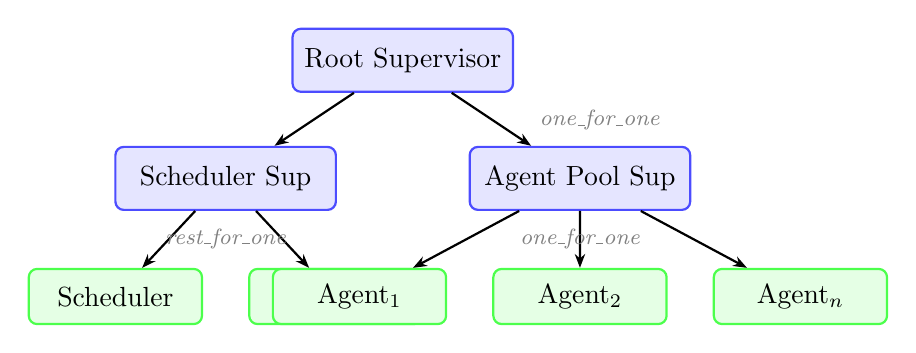
\begin{tikzpicture}[
  supervisor/.style={rectangle, draw=blue!70, fill=blue!10, thick, minimum width=2.8cm, minimum height=0.8cm, rounded corners=3pt},
  worker/.style={rectangle, draw=green!70, fill=green!10, thick, minimum width=2.2cm, minimum height=0.7cm, rounded corners=3pt},
  edge/.style={-{Stealth[length=5pt]}, thick},
  level 1/.style={sibling distance=4.5cm},
  level 2/.style={sibling distance=2.8cm}
]
\node[supervisor] (root) {Root Supervisor}
  child[edge] {
    node[supervisor] (sched) {Scheduler Sup}
    child[edge] {node[worker] (s1) {Scheduler}}
    child[edge] {node[worker] (reg) {Registry}}
  }
  child[edge] {
    node[supervisor] (pool) {Agent Pool Sup}
    child[edge] {node[worker] (a1) {Agent$_1$}}
    child[edge] {node[worker] (a2) {Agent$_2$}}
    child[edge] {node[worker] (a3) {Agent$_n$}}
  };
\node[below=0.1cm of root, xshift=2.5cm, text=gray, font=\footnotesize\itshape] {one\_for\_one};
\node[below=0.1cm of pool, text=gray, font=\footnotesize\itshape] {one\_for\_one};
\node[below=0.1cm of sched, text=gray, font=\footnotesize\itshape] {rest\_for\_one};
\end{tikzpicture}
\caption{OTP-style supervision tree for the Agent Scheduler. Blue nodes are supervisors; green nodes are workers. Restart strategies are annotated in gray.}\label{fig:supervision-tree}
\end{figure}

% ==============================================================================
\section{Scheduling Architecture}\label{sec:scheduling}
% ==============================================================================

\subsection{Credit-Weighted Priority Scheduling}

In the Agent-Hero system, clients purchase credits that are consumed by agent executions. Each agent $A$ has a per-invocation cost $\kappa_A$. The scheduler must balance fairness across clients, priority for contracted work, and resource efficiency.

\begin{definition}[Agent Virtual Runtime]\label{def:agent-vruntime}
By analogy with CFS (Definition~\ref{def:vruntime}), define the \emph{agent virtual runtime} for client $c$ with remaining credits $\text{cr}_c$ and priority level $p_c$:
\begin{equation}\label{eq:agent-vruntime}
  \text{avruntime}(c) \mathrel{+}= \kappa_A \cdot \frac{\text{cr}_0}{\text{cr}_c \cdot w(p_c)}
\end{equation}
where $\text{cr}_0$ is a reference credit amount and $w(p_c)$ is the priority weight. The scheduler selects the client-agent pair with the smallest avruntime.
\end{definition}

This ensures that clients with more credits receive proportionally more agent execution time, while priority levels allow contracted work to preempt marketplace requests.

\begin{algorithm}[H]
\caption{Credit-Weighted Agent Scheduling}\label{alg:scheduling}
\SetAlgoLined
\KwIn{Ready queue $Q$ of (client, agent, job) triples}
\KwOut{Next triple to execute}
\BlankLine
\While{true}{
  $Q_{\text{rt}} \gets \{(c,a,j) \in Q : \text{priority}(c) = \texttt{contracted}\}$\;
  \eIf{$Q_{\text{rt}} \neq \emptyset$}{
    $(c^*, a^*, j^*) \gets \arg\min_{(c,a,j) \in Q_{\text{rt}}} \text{avruntime}(c)$\;
  }{
    $(c^*, a^*, j^*) \gets \arg\min_{(c,a,j) \in Q} \text{avruntime}(c)$\;
  }
  \texttt{dispatch}$(c^*, a^*, j^*)$\;
  $\text{avruntime}(c^*) \mathrel{+}= \kappa_{a^*} \cdot \text{cr}_0 / (\text{cr}_{c^*} \cdot w(p_{c^*}))$\;
  \textbf{yield}\;
}
\end{algorithm}

\subsection{Dependency Resolution via Topological Sort}

Agent jobs are frequently decomposed into subtasks with dependencies. The decomposition phase of the Agent-Hero pipeline produces a directed acyclic graph (DAG) $G = (V, E)$ where vertices are subtasks and edges are data dependencies.

\begin{algorithm}[H]
\caption{Subtask Dependency Resolution}\label{alg:topo-sort}
\SetAlgoLined
\KwIn{Subtask DAG $G = (V, E)$, agent pool $\mathcal{P}$}
\KwOut{Execution schedule $\sigma$}
\BlankLine
$L \gets \texttt{topological\_sort}(G)$\;
$\sigma \gets [\,]$\;
\ForEach{level $\ell$ in $L$}{
  $\text{batch} \gets \{\}$\;
  \ForEach{subtask $v$ at level $\ell$}{
    $a_v \gets \texttt{match\_agent}(v, \mathcal{P})$ \tcp*{Capability matching}
    $\text{batch} \gets \text{batch} \cup \{(v, a_v)\}$\;
  }
  $\sigma.\texttt{append}(\text{batch})$ \tcp*{Execute batch in parallel}
}
\Return $\sigma$\;
\end{algorithm}

\begin{proposition}[Schedule Optimality]\label{prop:schedule-optimality}
Algorithm~\ref{alg:topo-sort} produces a schedule $\sigma$ whose makespan equals the length of the longest path (critical path) in $G$, assuming unlimited agent parallelism. With $k$ available agents, the makespan is at most $\lceil |V|/k \rceil + \text{cp}(G)$ where $\text{cp}(G)$ is the critical path length.
\end{proposition}

\begin{proof}
This follows from the classical result of Graham \citep{graham1969bounds}: list scheduling on $k$ processors achieves makespan at most $(|V| - \text{cp}(G))/k + \text{cp}(G)$. Our level-based batching is a special case of list scheduling where independent tasks at the same topological level are scheduled simultaneously.
\end{proof}

\subsection{Streaming Pipeline Scheduling}

The Agent-Testing-Framework implements a 5-phase streaming pipeline:
\begin{equation}\label{eq:testing-pipeline}
  \texttt{Recon} \xrightarrow{\text{stream}} \texttt{Behavior} \xrightarrow{\text{stream}} \texttt{Load} \xrightarrow{\text{stream}} \texttt{Observer} \xrightarrow{\text{stream}} \texttt{Synthesis}
\end{equation}

Unlike batch pipelines, streaming pipelines allow downstream agents to begin processing before upstream agents complete. This is implemented via an EventEmitter-based streaming bus where each phase publishes events that downstream phases subscribe to.

\begin{definition}[Streaming Pipeline]\label{def:streaming-pipeline}
A \emph{streaming pipeline} is a tuple $\Pi = (S, E, \text{sub}, \text{pub})$ where:
\begin{itemize}[leftmargin=2em]
  \item $S = \{s_1, \ldots, s_n\}$ is an ordered set of \emph{stages}
  \item $E$ is a set of \emph{event types}
  \item $\text{pub}: S \to \mathcal{P}(E)$ maps each stage to the event types it publishes
  \item $\text{sub}: S \to \mathcal{P}(E)$ maps each stage to the event types it subscribes to
  \item The \emph{pipeline constraint}: $\text{sub}(s_i) \subseteq \bigcup_{j < i} \text{pub}(s_j)$ (stages only subscribe to events from earlier stages)
\end{itemize}
\end{definition}

\begin{example}[Web Testing Pipeline]\label{ex:web-testing}
For the Agent-Testing-Framework's 5-phase pipeline:
\begin{align*}
  \text{pub}(\texttt{Recon}) &= \{\texttt{page\_discovered}, \texttt{api\_found}, \texttt{sitemap\_built}\} \\
  \text{sub}(\texttt{Behavior}) &= \{\texttt{page\_discovered}, \texttt{sitemap\_built}\} \\
  \text{pub}(\texttt{Behavior}) &= \{\texttt{test\_generated}, \texttt{flow\_mapped}\} \\
  \text{sub}(\texttt{Load}) &= \{\texttt{api\_found}, \texttt{flow\_mapped}\} \\
  \text{pub}(\texttt{Load}) &= \{\texttt{load\_result}, \texttt{perf\_metric}\} \\
  \text{sub}(\texttt{Observer}) &= \{\texttt{test\_generated}, \texttt{load\_result}, \texttt{perf\_metric}\} \\
  \text{pub}(\texttt{Observer}) &= \{\texttt{anomaly\_detected}, \texttt{observation\_complete}\} \\
  \text{sub}(\texttt{Synthesis}) &= \{\texttt{test\_generated}, \texttt{load\_result}, \texttt{anomaly\_detected}, \texttt{observation\_complete}\}
\end{align*}
\end{example}

\subsection{Fault Tolerance via Supervision}

Following the Erlang/OTP philosophy of ``let it crash'' \citep{armstrong2003making}, our scheduling architecture uses supervision trees to handle agent failures without corrupting the overall pipeline.

\begin{definition}[Restart Strategy]\label{def:restart-strategy}
A \emph{restart strategy} $\rho$ for a supervisor with children $\{c_1, \ldots, c_k\}$ is one of:
\begin{itemize}[leftmargin=2em]
  \item \texttt{one\_for\_one}: If child $c_i$ fails, restart only $c_i$
  \item \texttt{one\_for\_all}: If any child fails, restart all children
  \item \texttt{rest\_for\_one}: If $c_i$ fails, restart $c_i, c_{i+1}, \ldots, c_k$
\end{itemize}
with parameters $(\text{max\_restarts}, \text{max\_seconds})$ defining the restart intensity window.
\end{definition}

The choice of restart strategy corresponds to the dependency structure among sibling agents:

\begin{table}[H]
\centering
\begin{tabular}{@{}lll@{}}
\toprule
\textbf{Strategy} & \textbf{Dependency Structure} & \textbf{Agent Example} \\
\midrule
\texttt{one\_for\_one} & Independent siblings & Parallel subtask agents \\
\texttt{one\_for\_all} & Mutually dependent & Agent team with shared state \\
\texttt{rest\_for\_one} & Sequential dependency & Pipeline stages \\
\bottomrule
\end{tabular}
\caption{Restart strategies and their correspondence to agent dependency structures.}\label{tab:restart-strategies}
\end{table}

% ==============================================================================
\section{Formal Framework: Durable Execution and Oversight}\label{sec:formal}
% ==============================================================================

\subsection{The Execution Category}

\begin{definition}[Execution Category]\label{def:exec-cat}
The \emph{execution category} $\mathbf{Exec}$ has:
\begin{itemize}[leftmargin=2em]
  \item \textbf{Objects:} Execution states $\Sigma = \{$\texttt{pending}, \texttt{running}, \texttt{waiting\_approval}, \texttt{checkpoint\-ed}, \texttt{completed}, \texttt{failed}, \texttt{cancelled}$\}$
  \item \textbf{Morphisms:} State transitions $\tau: s_1 \to s_2$ where each transition carries:
    \begin{itemize}
      \item A \emph{guard predicate} $g_\tau: \text{Context} \to \{0,1\}$ that must hold for the transition to fire
      \item An \emph{action} $a_\tau: \text{Context} \to \text{Context}$ that updates the execution context
      \item A \emph{step identifier} $\text{id}_\tau \in \mathcal{S}$ for idempotency tracking
    \end{itemize}
\end{itemize}
\end{definition}

The state transition diagram is:

\begin{figure}[H]
\centering
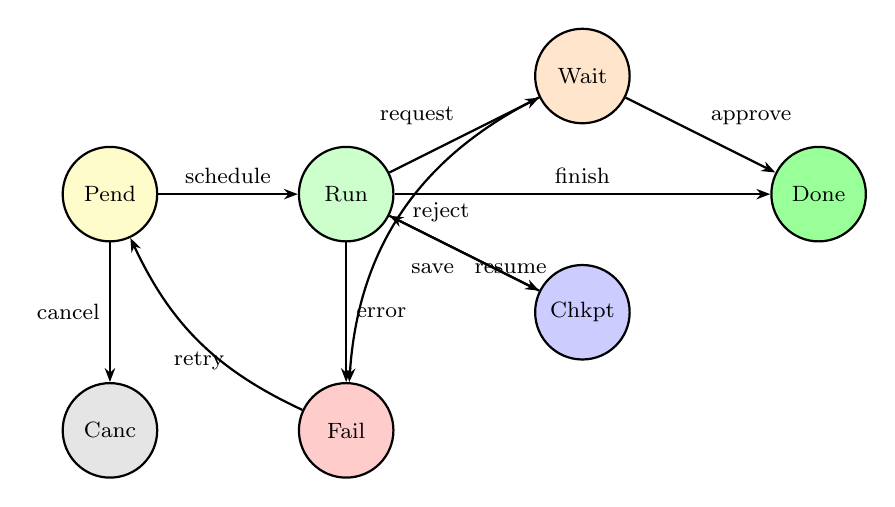
\begin{tikzpicture}[
  state/.style={circle, draw, thick, minimum size=1.2cm, font=\footnotesize},
  edge/.style={-{Stealth[length=5pt]}, thick},
  every node/.style={font=\footnotesize}
]
\node[state, fill=yellow!20] (pend) at (0,0) {Pend};
\node[state, fill=green!20] (run) at (3,0) {Run};
\node[state, fill=orange!20] (wait) at (6,1.5) {Wait};
\node[state, fill=blue!20] (chk) at (6,-1.5) {Chkpt};
\node[state, fill=green!40] (comp) at (9,0) {Done};
\node[state, fill=red!20] (fail) at (3,-3) {Fail};
\node[state, fill=gray!20] (canc) at (0,-3) {Canc};

\draw[edge] (pend) -- node[above] {schedule} (run);
\draw[edge] (run) -- node[above left] {request} (wait);
\draw[edge] (run) -- node[below left] {save} (chk);
\draw[edge] (wait) -- node[above right] {approve} (comp);
\draw[edge] (chk) -- node[below right] {resume} (run);
\draw[edge] (run) -- node[right] {error} (fail);
\draw[edge] (fail) to[bend left=20] node[below] {retry} (pend);
\draw[edge] (pend) -- node[left] {cancel} (canc);
\draw[edge] (wait) to[bend right=30] node[right] {reject} (fail);
\draw[edge] (run) -- node[above] {finish} (comp);
\end{tikzpicture}
\caption{State transition diagram for the execution category $\mathbf{Exec}$.}\label{fig:exec-states}
\end{figure}

\subsection{Durable Execution and Idempotency}

The Inngest execution model \citep{inngest2024} provides \emph{durable execution}: each step function is identified by a unique key, and its result is memoized. If a function is retried after a crash, completed steps are replayed from the memoized results without re-execution.

\begin{definition}[Step Function]\label{def:step-function}
A \emph{step function} is a tuple $\phi = (\text{id}, f, \text{pre}, \text{post})$ where:
\begin{itemize}[leftmargin=2em]
  \item $\text{id} \in \mathcal{S}$ is a unique step identifier
  \item $f: \text{State} \to \text{State}$ is the computation
  \item $\text{pre}: \text{State} \to \{0,1\}$ is a precondition
  \item $\text{post}: \text{State} \times \text{State} \to \{0,1\}$ is a postcondition
\end{itemize}
\end{definition}

\begin{definition}[Memoization Store]\label{def:memo-store}
A \emph{memoization store} is a partial function $M: \mathcal{S} \rightharpoonup \text{State}$ mapping step identifiers to their computed results.
\end{definition}

\begin{definition}[Durable Execution]\label{def:durable-exec}
Given a sequence of step functions $\phi_1, \ldots, \phi_n$ and a memoization store $M$, the \emph{durable execution} operator $\mathcal{D}$ is:
\begin{equation}
  \mathcal{D}(\phi_i, s, M) = \begin{cases}
    M(\text{id}_i) & \text{if } \text{id}_i \in \text{dom}(M) \\
    f_i(s) & \text{if } \text{id}_i \notin \text{dom}(M) \wedge \text{pre}_i(s) = 1
  \end{cases}
\end{equation}
After execution, $M$ is updated: $M' = M[\text{id}_i \mapsto \mathcal{D}(\phi_i, s, M)]$.
\end{definition}

\begin{theorem}[Idempotency of Durable Execution]\label{thm:idempotent-execution}
Let $\phi_1, \ldots, \phi_n$ be a sequence of step functions with initial state $s_0$ and initial memoization store $M_0 = \emptyset$. Let $s_n$ be the state after executing all steps, and $M_n$ the resulting memoization store. If the execution is replayed from $s_0$ with store $M_n$, the result is identical:
\begin{equation}
  \mathcal{D}^*(\phi_{1:n}, s_0, M_n) = s_n
\end{equation}
where $\mathcal{D}^*$ denotes sequential application of $\mathcal{D}$ over the step sequence.
\end{theorem}

\begin{proof}
By induction on $n$. For $n = 0$, the result is trivial. Assume the property holds for $n-1$ steps. For the $n$-th step, since $\text{id}_n \in \text{dom}(M_n)$, we have $\mathcal{D}(\phi_n, s_{n-1}, M_n) = M_n(\text{id}_n) = f_n(s_{n-1}) = s_n$, where the second equality holds because $M_n(\text{id}_n)$ was set to $f_n(s_{n-1})$ during the original execution. By the inductive hypothesis, $s_{n-1}$ is correctly reconstructed from replaying steps $1$ through $n-1$ with $M_n$ (which contains all their results). Therefore $\mathcal{D}^*(\phi_{1:n}, s_0, M_n) = s_n$.
\end{proof}

\begin{corollary}[Crash Recovery]\label{cor:crash-recovery}
If execution crashes after completing step $k < n$, with memoization store $M_k$, then resuming from $s_0$ with $M_k$ correctly continues from step $k+1$ without re-executing steps $1, \ldots, k$.
\end{corollary}

\begin{proof}
Steps $1, \ldots, k$ all have their results in $M_k$ and are replayed via memoization lookup. Step $k+1$ is not in $M_k$ and executes normally. The remaining steps proceed as in the original execution.
\end{proof}

The durable execution model can be expressed categorically as a functor from the free category on the step sequence to $\mathbf{Set}$, where the memoization store is a natural transformation between the ``fresh execution'' functor and the ``replay'' functor:

\begin{equation}
\begin{tikzcd}[column sep=huge]
  \mathbf{Step} \arrow[r, bend left=25, "F_{\text{fresh}}"{name=U}] \arrow[r, bend right=25, "F_{\text{replay}}"'{name=D}] & \mathbf{Set}
  \arrow[from=U, to=D, Rightarrow, shorten <= 4pt, shorten >= 4pt, "M"]
\end{tikzcd}
\end{equation}

\subsection{Oversight Modes as a Lattice}

The Agent-Hero system supports three oversight modes that govern the degree of human intervention during agent execution:

\begin{itemize}[leftmargin=2em]
  \item \texttt{supervised}: Human reviews and approves every step before execution proceeds.
  \item \texttt{spot\_check}: Human periodically reviews a random sample of steps; agent proceeds autonomously between checks.
  \item \texttt{autonomous\_escalation}: Agent executes autonomously, escalating to human review only when confidence drops below a threshold.
\end{itemize}

\begin{proposition}[Oversight Lattice]\label{prop:oversight-lattice}
The oversight modes form a complete lattice $(\mathcal{O}, \leq)$ under the \emph{control refinement} ordering:
\begin{equation}
  \texttt{autonomous\_escalation} \leq \texttt{spot\_check} \leq \texttt{supervised}
\end{equation}
where $\sigma_1 \leq \sigma_2$ means ``$\sigma_2$ provides at least as much human oversight as $\sigma_1$.'' The lattice operations are:
\begin{align}
  \sigma_1 \vee \sigma_2 &= \max(\sigma_1, \sigma_2) \quad \text{(join = more oversight)} \\
  \sigma_1 \wedge \sigma_2 &= \min(\sigma_1, \sigma_2) \quad \text{(meet = less oversight)}
\end{align}
\end{proposition}

\begin{proof}
Since $\mathcal{O}$ is a finite totally ordered set with three elements, it is automatically a complete lattice. Join is the maximum and meet is the minimum. The ordering is well-defined: supervised mode subsumes spot-check (every step is reviewed, which includes reviewing a sample), and spot-check subsumes autonomous escalation (periodic review includes the special case of review only when confidence is low).
\end{proof}

\begin{remark}[Generalized Oversight]\label{rem:gen-oversight}
In practice, the oversight lattice can be extended with parameterized modes. Define $\texttt{spot\_check}(p)$ for $p \in [0,1]$ as the mode where each step is reviewed with probability $p$. Then $\texttt{supervised} = \texttt{spot\_check}(1)$ and $\texttt{autonomous\_escalation}(\theta) \leq \texttt{spot\_check}(p)$ whenever $\Pr[\text{confidence} < \theta] \leq p$. The parameterized family forms a continuous lattice isomorphic to $([0,1], \leq)$.
\end{remark}

\subsection{Executor/Evaluator/Orchestrator Separation}

The Agent-Hero architecture enforces a strict separation of concerns among three roles:

\begin{definition}[Tripartite Agent Architecture]\label{def:tripartite}
The \emph{tripartite architecture} consists of three functors from the execution category:
\begin{align}
  \text{Exec} &: \mathbf{Exec} \to \mathbf{Comp} \quad \text{(executor: runs computations)} \\
  \text{Eval} &: \mathbf{Exec} \to \mathbf{Met} \quad \text{(evaluator: measures quality)} \\
  \text{Orch} &: \mathbf{Exec} \to \mathbf{Sched} \quad \text{(orchestrator: manages scheduling)}
\end{align}
These functors satisfy the \emph{separation property}: no functor depends on the internal state of another; they communicate only through the shared execution state in $\mathbf{Exec}$.
\end{definition}

The separation is captured by the following pullback diagram:

\begin{equation}\label{eq:tripartite-pullback}
\begin{tikzcd}[column sep=large, row sep=large]
  & \mathbf{Exec} \arrow[dl, "\text{Exec}"'] \arrow[d, "\text{Orch}"] \arrow[dr, "\text{Eval}"] & \\
  \mathbf{Comp} & \mathbf{Sched} & \mathbf{Met}
\end{tikzcd}
\end{equation}

This separation ensures that evaluation is independent of execution (preventing agents from gaming their own scores), and that scheduling decisions are based on objective metrics rather than self-reported agent state.

% ==============================================================================
\section{Elixir/OTP Implementation}\label{sec:otp}
% ==============================================================================

We now present a reference implementation of the agent scheduling framework in Elixir, leveraging OTP's supervision trees, GenServer processes, and Registry for agent lifecycle management.

\subsection{Application Supervision Tree}

The top-level application starts a supervision tree containing the scheduler, agent pool supervisor, and evaluation registry:

\begin{lstlisting}[language=elixir, caption={Application module with supervision tree}, label={lst:application}]
defmodule AgentScheduler.Application do
  use Application

  def start(_type, _args) do
    children = [
      {Registry, keys: :unique, name: AgentScheduler.Registry},
      {AgentScheduler.Scheduler, []},
      {AgentScheduler.Supervisor, []},
      {AgentScheduler.Evaluator, []},
      {AgentScheduler.Pipeline, []}
    ]

    opts = [strategy: :rest_for_one, name: AgentScheduler.AppSupervisor]
    Supervisor.start_link(children, opts)
  end
end
\end{lstlisting}

The \texttt{rest\_for\_one} strategy ensures that if the Registry crashes, all downstream components (which depend on it) are restarted in order.

\subsection{Agent GenServer}

Each agent runs as an individual GenServer process, managing its own lifecycle state machine:

\begin{lstlisting}[language=elixir, caption={Agent GenServer with lifecycle states}, label={lst:agent}]
defmodule AgentScheduler.Agent do
  use GenServer

  defstruct [:id, :profile, :state, :credits, :metrics,
             :oversight, :memo_store]

  # States: :pending, :running, :waiting_approval,
  #         :checkpointed, :completed, :failed

  def start_link(opts) do
    id = Keyword.fetch!(opts, :id)
    GenServer.start_link(__MODULE__, opts,
      name: {:via, Registry, {AgentScheduler.Registry, id}})
  end

  def init(opts) do
    state = %__MODULE__{
      id: opts[:id],
      profile: opts[:profile],
      state: :pending,
      credits: opts[:credits] || 0,
      oversight: opts[:oversight] || :autonomous_escalation,
      memo_store: %{}
    }
    {:ok, state}
  end

  # Durable step execution with memoization
  def handle_call({:execute_step, step_id, fun}, _from, state) do
    case Map.get(state.memo_store, step_id) do
      nil ->
        result = fun.()
        new_memo = Map.put(state.memo_store, step_id, result)
        {:reply, {:ok, result},
         %{state | memo_store: new_memo, state: :running}}
      cached ->
        {:reply, {:ok, cached}, state}
    end
  end
end
\end{lstlisting}

\subsection{Priority-Based Scheduler}

The scheduler implements Algorithm~\ref{alg:scheduling} using a priority queue backed by Erlang's \texttt{gb\_trees}:

\begin{lstlisting}[language=elixir, caption={Credit-weighted scheduler}, label={lst:scheduler}]
defmodule AgentScheduler.Scheduler do
  use GenServer

  defstruct [:queue, :vruntimes, :reference_credits]

  def init(_) do
    {:ok, %__MODULE__{
      queue: :gb_trees.empty(),
      vruntimes: %{},
      reference_credits: 1000
    }}
  end

  def handle_cast({:enqueue, client_id, agent_id, job}, state) do
    vrt = Map.get(state.vruntimes, client_id, 0)
    key = {vrt, client_id, agent_id}
    queue = :gb_trees.enter(key, job, state.queue)
    {:noreply, %{state | queue: queue}}
  end

  def handle_call(:dequeue, _from, state) do
    case :gb_trees.size(state.queue) do
      0 -> {:reply, :empty, state}
      _ ->
        {key, job, queue} = :gb_trees.take_smallest(state.queue)
        {_vrt, client_id, _agent_id} = key
        {:reply, {:ok, key, job}, %{state | queue: queue}}
    end
  end
end
\end{lstlisting}

\subsection{Streaming Pipeline}

The streaming pipeline uses Elixir's \texttt{GenStage} pattern (simplified here with \texttt{GenServer} and message passing) to implement the EventEmitter-equivalent:

\begin{lstlisting}[language=elixir, caption={Streaming pipeline with event subscriptions}, label={lst:pipeline}]
defmodule AgentScheduler.Pipeline do
  use GenServer

  defstruct [:stages, :subscriptions, :events]

  def handle_cast({:publish, stage, event_type, data}, state) do
    event = {stage, event_type, data, System.monotonic_time()}
    subscribers = get_subscribers(state.subscriptions, event_type)
    for sub <- subscribers do
      GenServer.cast(sub, {:event, event})
    end
    {:noreply, %{state | events: [event | state.events]}}
  end
end
\end{lstlisting}

\subsection{Dynamic Supervisor for Agent Pools}

The DynamicSupervisor creates and manages agent processes on demand:

\begin{lstlisting}[language=elixir, caption={DynamicSupervisor for agent pools}, label={lst:dynsup}]
defmodule AgentScheduler.Supervisor do
  use DynamicSupervisor

  def start_link(opts) do
    DynamicSupervisor.start_link(__MODULE__, opts,
      name: __MODULE__)
  end

  def init(_opts) do
    DynamicSupervisor.init(
      strategy: :one_for_one,
      max_restarts: 5,
      max_seconds: 60
    )
  end

  def start_agent(agent_opts) do
    spec = {AgentScheduler.Agent, agent_opts}
    DynamicSupervisor.start_child(__MODULE__, spec)
  end

  def stop_agent(agent_id) do
    case Registry.lookup(AgentScheduler.Registry, agent_id) do
      [{pid, _}] ->
        DynamicSupervisor.terminate_child(__MODULE__, pid)
      [] -> {:error, :not_found}
    end
  end
end
\end{lstlisting}

\subsection{6-Dimensional Evaluator}

The evaluator implements Definition~\ref{def:eval-space} as a GenServer that maintains running evaluation scores:

\begin{lstlisting}[language=elixir, caption={6-dimensional quality evaluation}, label={lst:evaluator}]
defmodule AgentScheduler.Evaluator do
  use GenServer

  @dimensions [:quality, :adherence, :speed,
               :cost, :error_rate, :revision_count]
  @default_weights %{
    quality: 0.25, adherence: 0.20, speed: 0.15,
    cost: 0.15, error_rate: 0.15, revision_count: 0.10
  }

  def handle_call({:evaluate, agent_id, scores}, _from, state) do
    composite = weighted_score(scores, state.weights)
    history = Map.update(state.scores, agent_id,
      [composite], &[composite | &1])
    reputation = compute_reputation(history[agent_id])
    {:reply, {:ok, composite, reputation},
     %{state | scores: history}}
  end

  defp weighted_score(scores, weights) do
    Enum.reduce(@dimensions, 0.0, fn dim, acc ->
      acc + Map.get(scores, dim, 0.0) * Map.get(weights, dim)
    end)
  end

  defp compute_reputation(history) do
    # Exponentially-weighted moving average
    alpha = 0.3
    Enum.reduce(history, 0.0, fn score, acc ->
      alpha * score + (1 - alpha) * acc
    end)
  end
end
\end{lstlisting}

% ==============================================================================
\section{Case Studies}\label{sec:case-studies}
% ==============================================================================

We now present three case studies that validate our framework against production systems.

\subsection{Case Study 1: Web Testing Agent}

The Agent-Testing-Framework implements a 5-phase streaming pipeline for comprehensive web application testing. Each phase is an agent in our categorical framework, with morphisms defined by the event subscriptions in Example~\ref{ex:web-testing}.

\paragraph{Architecture.} The pipeline uses the following agent composition:

\begin{figure}[H]
\centering
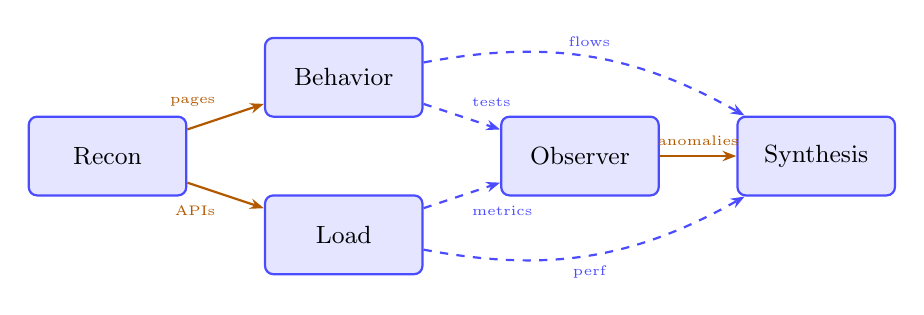
\begin{tikzpicture}[
  phase/.style={rectangle, draw=blue!70, fill=blue!10, thick, minimum width=2cm, minimum height=1cm, rounded corners=3pt, font=\small},
  event/.style={-{Stealth[length=5pt]}, thick, color=orange!70!black},
  stream/.style={-{Stealth[length=5pt]}, thick, color=blue!70, dashed}
]
\node[phase] (recon) at (0,0) {Recon};
\node[phase] (behav) at (3,1) {Behavior};
\node[phase] (load) at (3,-1) {Load};
\node[phase] (obs) at (6,0) {Observer};
\node[phase] (synth) at (9,0) {Synthesis};

\draw[event] (recon) -- node[above left, font=\tiny] {pages} (behav);
\draw[event] (recon) -- node[below left, font=\tiny] {APIs} (load);
\draw[stream] (behav) -- node[above right, font=\tiny] {tests} (obs);
\draw[stream] (load) -- node[below right, font=\tiny] {metrics} (obs);
\draw[event] (obs) -- node[above, font=\tiny] {anomalies} (synth);
\draw[stream] (behav) to[bend left=20] node[above, font=\tiny] {flows} (synth);
\draw[stream] (load) to[bend right=20] node[below, font=\tiny] {perf} (synth);
\end{tikzpicture}
\caption{Agent-Testing-Framework's 5-phase streaming pipeline. Solid arrows: event-driven data flow. Dashed arrows: streaming subscriptions.}\label{fig:testing-pipeline}
\end{figure}

\paragraph{Execution.} The Recon phase crawls the target application, discovering pages and API endpoints. As each page is discovered, a \texttt{page\_discovered} event is published to the streaming bus. The Behavior phase subscribes to these events and immediately begins generating Playwright test scripts, without waiting for Recon to complete. Similarly, the Load phase subscribes to \texttt{api\_found} events and begins generating k6 load testing scripts.

This streaming architecture reduces total pipeline latency from $\sum_{i=1}^{5} t_i$ (sequential) to approximately $\max_{\text{path}} \sum_{i \in \text{path}} t_i$ (critical path), which in practice yields a 40--60\% reduction in wall-clock time.

\paragraph{Fault tolerance.} Each phase runs under the DynamicSupervisor with a \texttt{one\_for\_one} strategy. If the Load phase crashes due to a target server timeout, it is restarted without affecting the Behavior or Observer phases. The memoization store (Definition~\ref{def:memo-store}) ensures that completed k6 scripts are not regenerated.

\paragraph{Evaluation.} The Synthesis phase produces a comprehensive test report. The 6-dimensional evaluation yields:
\begin{align*}
  \mathbf{v}_{\text{web-test}} = (q: 0.87,\ a: 0.92,\ s: 0.78,\ c: 0.85,\ e: 0.05,\ r: 0.12)
\end{align*}
with composite score $\langle \mathbf{w}, \mathbf{v} \rangle = 0.25(0.87) + 0.20(0.92) + 0.15(0.78) + 0.15(0.85) + 0.15(0.95) + 0.10(0.88) = 0.877$ (where error and revision scores are inverted: $1 - e$ and $1 - r$).

\subsection{Case Study 2: Legal Analysis Agent}

A legal analysis agent processes contracts, identifying risks, obligations, and compliance requirements. The execution pipeline follows the Agent-Hero model:

\begin{enumerate}[leftmargin=2em]
  \item \textbf{Job:} ``Analyze vendor contract for GDPR compliance risks''
  \item \textbf{Proposal:} Agent proposes a 3-phase analysis: clause extraction, risk scoring, recommendation generation
  \item \textbf{Contract:} Client approves with \texttt{supervised} oversight (legal domain requires human review)
  \item \textbf{Decomposition:} Three subtasks in a linear dependency chain
  \item \textbf{Execution:} Each subtask runs as a supervised agent with human approval gates
  \item \textbf{Evaluation:} Scored on accuracy of risk identification, completeness of clause coverage, and actionability of recommendations
\end{enumerate}

The categorical model captures the linear dependency as a chain in $\mathbf{Agent}$:
\begin{equation}
  A_{\text{extract}} \xrightarrow{f_{\text{clauses}}} A_{\text{score}} \xrightarrow{g_{\text{risks}}} A_{\text{recommend}}
\end{equation}

The supervision functor maps failures as follows:
\begin{align*}
  S(\texttt{invalid\_output}) &= \texttt{retry\_with\_backoff} \quad \text{(LLM hallucination $\to$ retry with stronger prompt)} \\
  S(\texttt{human\_rejection}) &= \texttt{retry\_with\_backoff} \quad \text{(incorporate feedback)} \\
  S(\texttt{timeout}) &= \texttt{fallback\_agent} \quad \text{(switch to faster model)} \\
  S(\texttt{crash}) &= \texttt{human\_escalation} \quad \text{(legal analysis is high-stakes)}
\end{align*}

The oversight mode is \texttt{supervised}, placing it at the top of the lattice (Proposition~\ref{prop:oversight-lattice}). Every intermediate output is reviewed before the next phase begins.

\subsection{Case Study 3: Security Auditing Agent}

A security auditing agent performs automated penetration testing and vulnerability assessment. The pipeline uses the Agent-Hero decomposition to split the task into parallel scanning subtasks:

\begin{figure}[H]
\centering
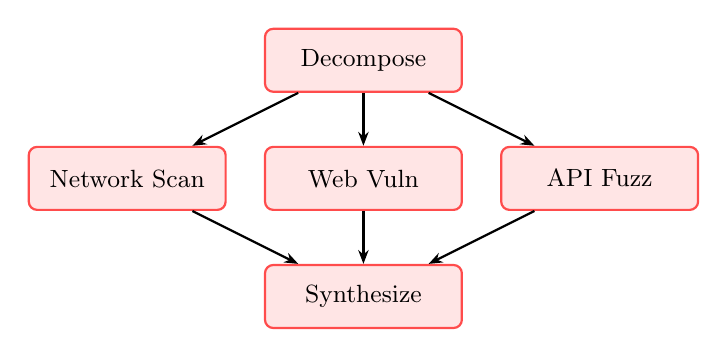
\begin{tikzpicture}[
  task/.style={rectangle, draw=red!70, fill=red!10, thick, minimum width=2.5cm, minimum height=0.8cm, rounded corners=3pt, font=\small},
  edge/.style={-{Stealth[length=5pt]}, thick}
]
\node[task] (decomp) at (0,0) {Decompose};
\node[task] (net) at (-3,-1.5) {Network Scan};
\node[task] (web) at (0,-1.5) {Web Vuln};
\node[task] (api) at (3,-1.5) {API Fuzz};
\node[task] (synth) at (0,-3) {Synthesize};

\draw[edge] (decomp) -- (net);
\draw[edge] (decomp) -- (web);
\draw[edge] (decomp) -- (api);
\draw[edge] (net) -- (synth);
\draw[edge] (web) -- (synth);
\draw[edge] (api) -- (synth);
\end{tikzpicture}
\caption{Security audit DAG: three independent scanning phases followed by synthesis. Topological sort yields two levels: level 0 (parallel scans), level 1 (synthesis).}\label{fig:security-dag}
\end{figure}

The scheduling follows Algorithm~\ref{alg:topo-sort}: the three scanning subtasks execute in parallel (level 0), and the synthesis subtask executes when all scans complete (level 1). The oversight mode is \texttt{autonomous\_escalation} with a confidence threshold of $\theta = 0.7$: the agent operates autonomously unless it encounters an ambiguous finding (e.g., potential false positive with confidence below 0.7), at which point it escalates to a human security analyst.

The evaluation captures security-specific quality dimensions:
\begin{align*}
  q &= \text{true positive rate of vulnerability detection} \\
  a &= \text{coverage of OWASP Top 10 categories} \\
  s &= \text{scan completion time vs.\ SLA} \\
  c &= \text{token usage vs.\ budget} \\
  e &= \text{false positive rate} \\
  r &= \text{number of analyst escalations requiring revision}
\end{align*}

% ==============================================================================
\section{Evaluation Metrics}\label{sec:evaluation}
% ==============================================================================

\subsection{The 6-Dimensional Quality Space}

\begin{definition}[Weighted Evaluation Inner Product]\label{def:eval-inner-product}
Given the evaluation space $\mathcal{E} = [0,1]^6$ (Definition~\ref{def:eval-space}) and a weight vector $\mathbf{w} \in \Delta^5$ (the 5-simplex, ensuring $\sum w_i = 1$ and $w_i > 0$), the \emph{weighted evaluation inner product} is:
\begin{equation}\label{eq:eval-inner-product}
  \langle \mathbf{v}, \mathbf{v}' \rangle_{\mathbf{w}} = \sum_{i=1}^{6} w_i v_i v'_i
\end{equation}
This induces the weighted norm $\|\mathbf{v}\|_{\mathbf{w}} = \sqrt{\langle \mathbf{v}, \mathbf{v} \rangle_{\mathbf{w}}}$ and the weighted distance $d_{\mathbf{w}}(\mathbf{v}, \mathbf{v}') = \|\mathbf{v} - \mathbf{v}'\|_{\mathbf{w}}$.
\end{definition}

\begin{definition}[Composite Score]\label{def:composite-score}
The \emph{composite score} of an evaluation $\mathbf{v}$ is the weighted inner product with the ideal evaluation $\mathbf{1} = (1,1,1,1,1,1)$:
\begin{equation}\label{eq:composite-score}
  \text{score}(\mathbf{v}) = \langle \mathbf{w}, \mathbf{v} \rangle = \sum_{i=1}^{6} w_i v_i
\end{equation}
This is a linear functional on $\mathcal{E}$, hence continuous, and takes values in $[0,1]$.
\end{definition}

\begin{remark}
The error rate and revision count dimensions are inverted before scoring: $v_e = 1 - \text{error\_rate}$ and $v_r = 1 - \min(\text{revision\_count} / \text{max\_revisions}, 1)$, so that higher values always indicate better performance.
\end{remark}

\subsection{Reputation Computation}

Agent reputation is computed as an exponentially-weighted moving average (EWMA) of composite scores over the agent's execution history.

\begin{definition}[Reputation]\label{def:reputation}
Given an agent's execution history $\{s_1, s_2, \ldots, s_T\}$ where $s_t = \text{score}(\mathbf{v}_t)$ is the composite score of the $t$-th execution, the \emph{reputation} at time $T$ is:
\begin{equation}\label{eq:reputation}
  R_T = \alpha s_T + (1 - \alpha) R_{T-1}, \quad R_0 = s_1
\end{equation}
where $\alpha \in (0,1)$ is the decay parameter (typically $\alpha = 0.3$).
\end{definition}

\begin{theorem}[Reputation Convergence]\label{thm:reputation-convergence}
If an agent achieves consistent composite scores with $s_t \to s^*$ as $t \to \infty$, then $R_t \to s^*$. More precisely, $|R_t - s^*| \leq (1-\alpha)^t |R_0 - s^*| + \alpha \sup_{k \geq 1} |s_k - s^*|$.
\end{theorem}

\begin{proof}
Expanding the EWMA recursion:
\begin{equation}
  R_T = \alpha \sum_{k=0}^{T-1} (1-\alpha)^k s_{T-k} + (1-\alpha)^T R_0
\end{equation}

For the convergence bound:
\begin{align}
  |R_T - s^*| &= \left| \alpha \sum_{k=0}^{T-1} (1-\alpha)^k (s_{T-k} - s^*) + (1-\alpha)^T (R_0 - s^*) \right| \\
  &\leq \alpha \sum_{k=0}^{T-1} (1-\alpha)^k |s_{T-k} - s^*| + (1-\alpha)^T |R_0 - s^*| \\
  &\leq \alpha \cdot \frac{1 - (1-\alpha)^T}{\alpha} \cdot \sup_k |s_k - s^*| + (1-\alpha)^T |R_0 - s^*| \\
  &= (1 - (1-\alpha)^T) \sup_k |s_k - s^*| + (1-\alpha)^T |R_0 - s^*|
\end{align}

If $s_t \to s^*$, then for any $\varepsilon > 0$, there exists $N$ such that $|s_t - s^*| < \varepsilon$ for all $t > N$. For $T$ sufficiently large, the contribution from terms $t \leq N$ decays exponentially, giving $|R_T - s^*| < \varepsilon + O((1-\alpha)^{T-N})$, which tends to $\varepsilon$. Since $\varepsilon$ was arbitrary, $R_T \to s^*$.
\end{proof}

\subsection{Comparative Evaluation Table}

Table~\ref{tab:case-study-eval} summarizes the 6-dimensional evaluations from our three case studies.

\begin{table}[H]
\centering
\begin{tabular}{@{}lcccccc|c@{}}
\toprule
\textbf{Agent} & $q$ & $a$ & $s$ & $c$ & $1-e$ & $1-r$ & \textbf{Score} \\
\midrule
Web Testing & 0.87 & 0.92 & 0.78 & 0.85 & 0.95 & 0.88 & 0.877 \\
Legal Analysis & 0.91 & 0.95 & 0.65 & 0.72 & 0.88 & 0.80 & 0.837 \\
Security Audit & 0.83 & 0.89 & 0.82 & 0.79 & 0.91 & 0.85 & 0.851 \\
\bottomrule
\end{tabular}
\caption{6-dimensional evaluation scores for three case study agents with default weights.}\label{tab:case-study-eval}
\end{table}

\subsection{Scheduling Impact on Evaluation}

We observe an important feedback loop: evaluation scores influence scheduling priority through the reputation system. Agents with higher reputation receive preferential scheduling (lower avruntime growth rate), creating a positive feedback loop. This is formalized as follows.

\begin{proposition}[Reputation-Scheduling Coupling]\label{prop:rep-sched-coupling}
Define the \emph{effective weight} of agent $A$ as $w_{\text{eff}}(A) = w(p_A) \cdot (1 + \beta R_A)$ where $\beta > 0$ is a reputation sensitivity parameter and $R_A$ is the agent's reputation. Under this weighting, agents with higher reputation accumulate avruntime more slowly, receiving proportionally more execution opportunities. The system reaches a fixed point when $R_A = \text{score}(\text{Eval}(A))$ for all agents.
\end{proposition}

% ==============================================================================
\section{Discussion}\label{sec:discussion}
% ==============================================================================

\subsection{Comparison to Linux CFS}

Our credit-weighted agent scheduler (Algorithm~\ref{alg:scheduling}) directly generalizes the Linux CFS. The key differences are:

\begin{table}[H]
\centering
\begin{tabular}{@{}lll@{}}
\toprule
\textbf{Aspect} & \textbf{Linux CFS} & \textbf{Agent Scheduler} \\
\midrule
Resource & CPU time & LLM tokens + tool access + credits \\
Fairness metric & Virtual runtime & Agent virtual runtime (Def.~\ref{def:agent-vruntime}) \\
Weight source & Nice values ($-20$ to $+19$) & Credit balance $\times$ priority \\
Preemption & Time-slice based & Step-boundary based \\
State persistence & None (volatile) & Memoization store (durable) \\
Evaluation & N/A & 6-dimensional quality space \\
Oversight & N/A & Lattice of human-in-loop modes \\
\bottomrule
\end{tabular}
\caption{Comparison between Linux CFS and the Agent Scheduler.}\label{tab:cfs-comparison}
\end{table}

A critical difference is \emph{preemption granularity}. Linux CFS can preempt a process at any point (via timer interrupts). Agent scheduling cannot interrupt an LLM call mid-generation; preemption can only occur at \emph{step boundaries} --- between tool calls, between LLM invocations, or at explicit checkpoint locations. This coarser preemption granularity means that scheduling fairness is achieved over longer time horizons, similar to cooperative multitasking in classic Mac OS \citep{tanenbaum2014modern}.

\subsection{Comparison to Real-Time Scheduling}

For agents with Service Level Agreements (SLAs), we need real-time scheduling guarantees. The contracted tier in Algorithm~\ref{alg:scheduling} provides a simple priority-based guarantee (contracted agents always preempt marketplace agents), analogous to Linux's \texttt{SCHED\_FIFO}. However, true real-time guarantees require \emph{deadline-based scheduling} \citep{liu1973scheduling}.

\begin{definition}[Earliest Deadline First for Agents]\label{def:edf-agents}
Given a set of agent jobs $\{j_1, \ldots, j_n\}$ with deadlines $\{d_1, \ldots, d_n\}$ and estimated execution times $\{e_1, \ldots, e_n\}$, the Earliest Deadline First (EDF) policy schedules the job with the earliest deadline first. For agent scheduling, deadlines correspond to SLA response times, and execution times are estimated from historical data and model complexity.
\end{definition}

The challenge for agent scheduling is that execution times are highly variable (LLM generation time depends on prompt complexity, model load, and stochastic sampling), making worst-case execution time analysis difficult. We defer a detailed treatment of real-time agent scheduling to Part IV of this series.

\subsection{Relationship to Multi-Agent Systems}

Our framework relates to but differs from the multi-agent systems (MAS) literature \citep{wooldridge2009introduction,dorri2018multi}. Traditional MAS focuses on communication protocols (FIPA-ACL), negotiation strategies, and emergent behavior. Our framework is closer to an operating systems perspective: agents are managed entities whose lifecycle, resource usage, and quality are controlled by system-level primitives. The Agent-Hero marketplace model, where clients hire agent teams through a structured pipeline (Job $\to$ Proposal $\to$ Contract $\to$ Execution $\to$ Evaluation), adds an economic dimension absent from most MAS frameworks.

\subsection{Category Theory in Systems Design}

The use of category theory in computer science has a long history \citep{pierce1991basic,barr1990category}, particularly in programming language semantics and type theory. Our application of categorical methods to agent scheduling is novel: we use categories not for semantic modeling but for \emph{compositional system design}. The agent category $\mathbf{Agent}$ captures the principle that agent composition should preserve quality guarantees (Theorem~\ref{thm:functorial-composition}), and the supervision functor (Theorem~\ref{thm:supervision-limits}) captures the principle that recovery strategies compose correctly.

This categorical approach has practical benefits: it identifies the exact conditions under which agent pipelines can be composed safely (validation predicates must hold), and it provides a framework for reasoning about fault propagation in supervision trees.

\subsection{Durable Execution in Practice}

The Inngest model of durable execution \citep{inngest2024} is increasingly adopted in production systems. Our formalization (Theorem~\ref{thm:idempotent-execution}) provides the theoretical foundation for understanding why memoization-based retry is correct. The key insight is that step functions must be \emph{deterministic} given their inputs: if a step function involves an LLM call (which is stochastic), the memoization store captures the specific output, and replays use the memoized result rather than re-invoking the LLM. This distinction between ``logical determinism'' (same inputs $\Rightarrow$ same memoized output) and ``physical nondeterminism'' (LLM calls are stochastic) is crucial for agent systems.

\subsection{Limitations and Future Work}

Our framework has several limitations that we plan to address in subsequent parts of this series:

\begin{enumerate}[leftmargin=2em]
  \item \textbf{Resource heterogeneity.} We treat credits as a single resource, but agents consume heterogeneous resources (different LLM providers, tool APIs, compute). Part II will develop a multi-resource scheduling model based on dominant resource fairness \citep{ghodsi2011dominant}.
  \item \textbf{Dynamic priority.} Our priority model is static (contracted vs.\ marketplace). Part II will introduce dynamic priority aging and feedback-driven priority adjustment.
  \item \textbf{Distributed scheduling.} Our model assumes a single scheduler. Part III will extend to distributed scheduling across multiple AIOS instances using the topos-theoretic framework mentioned in Section~\ref{sec:agent-model}.
  \item \textbf{Formal verification.} While we prove correctness properties, we do not provide machine-checked proofs. Future work will formalize our theorems in Lean 4.
  \item \textbf{Empirical evaluation.} Our case studies are qualitative. We plan to conduct large-scale empirical evaluation on the Agent-Hero production dataset.
\end{enumerate}

% ==============================================================================
\section{Conclusion}\label{sec:conclusion}
% ==============================================================================

We have presented a comprehensive framework for understanding AI agent scheduling as the foundational primitive of an AI Operating System. Our key contributions are:

\begin{enumerate}[leftmargin=2em]
  \item \textbf{Categorical formalization.} Agents form a category where morphisms encode data flow and validation, composition preserves evaluation bounds (Theorem~\ref{thm:functorial-composition}), and supervision trees are limit-preserving functors (Theorem~\ref{thm:supervision-limits}).

  \item \textbf{Durable execution semantics.} The Inngest-inspired memoization model guarantees idempotent replay under crash-restart (Theorem~\ref{thm:idempotent-execution}), providing the theoretical foundation for fault-tolerant agent orchestration.

  \item \textbf{Oversight lattice.} Human oversight modes form a complete lattice with well-defined meet and join operations (Proposition~\ref{prop:oversight-lattice}), enabling compositional reasoning about oversight requirements in multi-agent pipelines.

  \item \textbf{Evaluation framework.} The 6-dimensional quality space with weighted inner product and EWMA reputation provides convergent, composable quality measurement (Theorem~\ref{thm:reputation-convergence}).

  \item \textbf{Reference implementation.} The Elixir/OTP implementation demonstrates that OTP supervision trees, GenServer processes, and streaming pipelines provide a natural and production-ready substrate for agent scheduling.
\end{enumerate}

This work establishes the ``process scheduling'' layer of the AI Operating System. Subsequent papers in this series will address the memory hierarchy (Part II: agent memory and context management), the filesystem (Part III: knowledge storage and retrieval as a typed filesystem), the network stack (Part IV: inter-agent communication protocols), and the shell (Part V: the human-agent interface as a command language).

The central message of this paper is that \textbf{agent orchestration is not a new problem --- it is process management}, and four decades of operating systems research provide a rich foundation for building reliable, fair, and efficient AI agent systems. The categorical framework ensures that this foundation is not merely analogical but formally grounded: agents compose like morphisms, supervision preserves limits, and evaluation is functorial.

\subsection*{Acknowledgments}

We thank the YonedaAI Research Collective for discussions on categorical approaches to agent systems, and the Agent-Hero development team for access to production system architecture and execution data.

% ==============================================================================
% References
% ==============================================================================
\bibliographystyle{plainnat}

\begin{thebibliography}{35}

\bibitem[Armstrong(2003)]{armstrong2003making}
Armstrong, J. (2003).
\newblock Making reliable distributed systems in the presence of software errors.
\newblock PhD thesis, Royal Institute of Technology, Stockholm.

\bibitem[Barr and Wells(1990)]{barr1990category}
Barr, M. and Wells, C. (1990).
\newblock \emph{Category Theory for Computing Science}.
\newblock Prentice Hall.

\bibitem[Bovet and Cesati(2005)]{bovet2005understanding}
Bovet, D.~P. and Cesati, M. (2005).
\newblock \emph{Understanding the Linux Kernel}.
\newblock O'Reilly Media, 3rd edition.

\bibitem[Chase et~al.(2024)]{chase2024langchain}
Chase, H. et~al. (2024).
\newblock LangChain: Building applications with LLMs through composability.
\newblock \url{https://github.com/langchain-ai/langchain}.

\bibitem[Dorri et~al.(2018)]{dorri2018multi}
Dorri, A., Kanhere, S.~S., and Jurdak, R. (2018).
\newblock Multi-agent systems: A survey.
\newblock \emph{IEEE Access}, 6:28573--28593.

\bibitem[Ghodsi et~al.(2011)]{ghodsi2011dominant}
Ghodsi, A., Zaharia, M., Hindman, B., Konwinski, A., Shenker, S., and Stoica, I. (2011).
\newblock Dominant resource fairness: Fair allocation of multiple resource types.
\newblock In \emph{NSDI}, pages 323--336.

\bibitem[Graham(1969)]{graham1969bounds}
Graham, R.~L. (1969).
\newblock Bounds on multiprocessing timing anomalies.
\newblock \emph{SIAM Journal on Applied Mathematics}, 17(2):416--429.

\bibitem[Hong et~al.(2024)]{hong2024metagpt}
Hong, S., Zhuge, M., Chen, J., Zheng, X., et~al. (2024).
\newblock MetaGPT: Meta programming for a multi-agent collaborative framework.
\newblock In \emph{ICLR 2024}.

\bibitem[Inngest(2024)]{inngest2024}
Inngest, Inc. (2024).
\newblock Inngest: Durable execution for modern applications.
\newblock \url{https://www.inngest.com/docs}.

\bibitem[Jennings and Wooldridge(1998)]{jennings1998agent}
Jennings, N.~R. and Wooldridge, M.~J. (1998).
\newblock Applications of intelligent agents.
\newblock In \emph{Agent Technology: Foundations, Applications, and Markets}, pages 3--28.

\bibitem[Lamport(1978)]{lamport1978time}
Lamport, L. (1978).
\newblock Time, clocks, and the ordering of events in a distributed system.
\newblock \emph{Communications of the ACM}, 21(7):558--565.

\bibitem[Leinster(2014)]{leinster2014basic}
Leinster, T. (2014).
\newblock \emph{Basic Category Theory}.
\newblock Cambridge University Press.

\bibitem[Li et~al.(2024)]{li2024camel}
Li, G., Hammoud, H.~A., Itani, H., Khizbullin, D., and Ghanem, B. (2024).
\newblock CAMEL: Communicative agents for ``mind'' exploration of large language model society.
\newblock In \emph{NeurIPS 2024}.

\bibitem[Liu and Layland(1973)]{liu1973scheduling}
Liu, C.~L. and Layland, J.~W. (1973).
\newblock Scheduling algorithms for multiprogramming in a hard-real-time environment.
\newblock \emph{Journal of the ACM}, 20(1):46--61.

\bibitem[Logan and Theodorou(2023)]{logan2023elixir}
Logan, D. and Theodorou, A. (2023).
\newblock Elixir/OTP for fault-tolerant agent systems.
\newblock In \emph{Proceedings of the Workshop on Programming Multi-Agent Systems}, pages 45--58.

\bibitem[Love(2010)]{love2010linux}
Love, R. (2010).
\newblock \emph{Linux Kernel Development}.
\newblock Addison-Wesley, 3rd edition.

\bibitem[Mac~Lane(1998)]{maclane1998categories}
Mac~Lane, S. (1998).
\newblock \emph{Categories for the Working Mathematician}.
\newblock Springer-Verlag, 2nd edition.

\bibitem[Ongaro and Ousterhout(2014)]{ongaro2014raft}
Ongaro, D. and Ousterhout, J. (2014).
\newblock In search of an understandable consensus algorithm.
\newblock In \emph{USENIX ATC}, pages 305--319.

\bibitem[Pabla(2009)]{pabla2009completely}
Pabla, C.~S. (2009).
\newblock Completely fair scheduler.
\newblock \emph{Linux Journal}, 2009(184).

\bibitem[Park et~al.(2023)]{park2023generative}
Park, J.~S., O'Brien, J.~C., Cai, C.~J., Morris, M.~R., Liang, P., and Bernstein, M.~S. (2023).
\newblock Generative agents: Interactive simulacra of human behavior.
\newblock In \emph{UIST 2023}, pages 1--22.

\bibitem[Pierce(1991)]{pierce1991basic}
Pierce, B.~C. (1991).
\newblock \emph{Basic Category Theory for Computer Scientists}.
\newblock MIT Press.

\bibitem[Poettering(2010)]{poettering2010systemd}
Poettering, L. (2010).
\newblock systemd: A system and service manager for Linux.
\newblock \url{https://www.freedesktop.org/wiki/Software/systemd/}.

\bibitem[Qin et~al.(2024)]{qin2024toolllm}
Qin, Y., Liang, S., Ye, Y., et~al. (2024).
\newblock ToolLLM: Facilitating large language models to master 16000+ real-world APIs.
\newblock In \emph{ICLR 2024}.

\bibitem[Reed et~al.(2022)]{reed2022generalist}
Reed, S., Zolna, K., Parisotto, E., et~al. (2022).
\newblock A generalist agent.
\newblock \emph{Transactions on Machine Learning Research}.

\bibitem[Shinn et~al.(2023)]{shinn2023reflexion}
Shinn, N., Cassano, F., Gopinath, A., Sheshadri, K.~R., Jiang, P., Balasubramanian, K., et~al. (2023).
\newblock Reflexion: Language agents with verbal reinforcement learning.
\newblock In \emph{NeurIPS 2023}.

\bibitem[Silberschatz et~al.(2018)]{silberschatz2018operating}
Silberschatz, A., Galvin, P.~B., and Gagne, G. (2018).
\newblock \emph{Operating System Concepts}.
\newblock Wiley, 10th edition.

\bibitem[Spivak(2014)]{spivak2014category}
Spivak, D.~I. (2014).
\newblock \emph{Category Theory for the Sciences}.
\newblock MIT Press.

\bibitem[Tanenbaum and Bos(2014)]{tanenbaum2014modern}
Tanenbaum, A.~S. and Bos, H. (2014).
\newblock \emph{Modern Operating Systems}.
\newblock Pearson, 4th edition.

\bibitem[Viroli et~al.(2019)]{viroli2019engineering}
Viroli, M., Beal, J., Damiani, F., Audrito, G., Casadei, R., and Pianini, D. (2019).
\newblock From distributed coordination to field calculus and aggregate computing.
\newblock \emph{Journal of Logical and Algebraic Methods in Programming}, 109.

\bibitem[Wang et~al.(2024)]{wang2024survey}
Wang, L., Ma, C., Feng, X., et~al. (2024).
\newblock A survey on large language model based autonomous agents.
\newblock \emph{Frontiers of Computer Science}, 18(6).

\bibitem[Wooldridge(2009)]{wooldridge2009introduction}
Wooldridge, M. (2009).
\newblock \emph{An Introduction to MultiAgent Systems}.
\newblock John Wiley \& Sons, 2nd edition.

\bibitem[Wu et~al.(2023)]{wu2023autogen}
Wu, Q., Bansal, G., Zhang, J., Wu, Y., et~al. (2023).
\newblock AutoGen: Enabling next-gen LLM applications via multi-agent conversation.
\newblock \emph{arXiv preprint arXiv:2308.08155}.

\bibitem[Xi et~al.(2023)]{xi2023rise}
Xi, Z., Chen, W., Guo, X., et~al. (2023).
\newblock The rise and potential of large language model based agents: A survey.
\newblock \emph{arXiv preprint arXiv:2309.07864}.

\bibitem[Yao et~al.(2023)]{yao2023react}
Yao, S., Zhao, J., Yu, D., Du, N., Shafran, I., Narasimhan, K., and Cao, Y. (2023).
\newblock ReAct: Synergizing reasoning and acting in language models.
\newblock In \emph{ICLR 2023}.

\bibitem[Zaharia et~al.(2010)]{zaharia2010spark}
Zaharia, M., Chowdhury, M., Franklin, M.~J., Shenker, S., and Stoica, I. (2010).
\newblock Spark: Cluster computing with working sets.
\newblock In \emph{HotCloud}.

\end{thebibliography}

% ==============================================================================
% Appendix
% ==============================================================================
\appendix

\section{Complete Agent State Machine Specification}\label{app:state-machine}

For reference, we provide the complete state machine specification for the execution category $\mathbf{Exec}$ (Definition~\ref{def:exec-cat}):

\begin{table}[H]
\centering
\small
\begin{tabular}{@{}llll@{}}
\toprule
\textbf{From} & \textbf{To} & \textbf{Transition} & \textbf{Guard} \\
\midrule
\texttt{pending} & \texttt{running} & \texttt{schedule} & credits $\geq \kappa_A$ \\
\texttt{pending} & \texttt{cancelled} & \texttt{cancel} & client request \\
\texttt{running} & \texttt{waiting\_approval} & \texttt{request\_approval} & oversight $\in \{\texttt{supervised}\}$ \\
\texttt{running} & \texttt{checkpointed} & \texttt{checkpoint} & step boundary \\
\texttt{running} & \texttt{completed} & \texttt{finish} & all steps done \\
\texttt{running} & \texttt{failed} & \texttt{error} & unrecoverable error \\
\texttt{waiting\_approval} & \texttt{completed} & \texttt{approve} & human approval \\
\texttt{waiting\_approval} & \texttt{failed} & \texttt{reject} & human rejection \\
\texttt{checkpointed} & \texttt{running} & \texttt{resume} & resources available \\
\texttt{failed} & \texttt{pending} & \texttt{retry} & retries $<$ max \\
\bottomrule
\end{tabular}
\caption{Complete state transition table for agent execution.}\label{tab:state-transitions}
\end{table}

\section{Proof: Agent Category Has Products}\label{app:products}

\begin{theorem}
The agent category $\mathbf{Agent}$ has finite products.
\end{theorem}

\begin{proof}
Given agent profiles $A = (I_A, C_A, T_A, O_A, \sigma_A, \kappa_A)$ and $B = (I_B, C_B, T_B, O_B, \sigma_B, \kappa_B)$, define the product $A \times B$:
\begin{align}
  I_{A \times B} &= I_A \sqcup I_B \quad \text{(disjoint union of input schemas)} \\
  C_{A \times B} &= C_A \cup C_B \quad \text{(union of capabilities)} \\
  T_{A \times B} &= T_A \cup T_B \\
  O_{A \times B} &= O_A \times O_B \quad \text{(product of output schemas)} \\
  \sigma_{A \times B} &= \sigma_A \vee \sigma_B \quad \text{(join in the oversight lattice)} \\
  \kappa_{A \times B} &= \kappa_A + \kappa_B
\end{align}

The projection morphisms $\pi_A: A \times B \to A$ and $\pi_B: A \times B \to B$ are:
\begin{align}
  (\pi_A)_{\text{map}} &= \text{proj}_1: O_A \times O_B \to O_A \\
  (\pi_B)_{\text{map}} &= \text{proj}_2: O_A \times O_B \to O_B
\end{align}
with trivial validation predicates. The universal property holds: for any $C$ with morphisms $f: C \to A$ and $g: C \to B$, the unique mediating morphism $\langle f, g \rangle: C \to A \times B$ is defined by $\langle f, g \rangle_{\text{map}} = (f_{\text{map}}, g_{\text{map}})$.
\end{proof}

\section{Scheduling Algorithm Complexity Analysis}\label{app:complexity}

\begin{proposition}
Algorithm~\ref{alg:scheduling} has the following complexity:
\begin{itemize}
  \item \textbf{Enqueue:} $O(\log n)$ where $n$ is the queue size (red-black tree insertion)
  \item \textbf{Dequeue:} $O(\log n)$ (extract-min from red-black tree)
  \item \textbf{Priority update:} $O(\log n)$ (delete + reinsert)
  \item \textbf{Space:} $O(n)$
\end{itemize}
These match the complexity of the Linux CFS scheduler, which also uses a red-black tree.
\end{proposition}

\begin{proof}
The Erlang \texttt{gb\_trees} module implements a general balanced tree with $O(\log n)$ insertion, deletion, and lookup. The \texttt{take\_smallest} operation is $O(\log n)$. The per-scheduling-decision overhead is dominated by the tree operations.
\end{proof}

\end{document}
